% Copyright 2004 Alexander Grahn
%
% This material is subject to the LaTeX Project Public License. See
%    http://www.ctan.org/tex-archive/help/Catalogue/licenses.lppl.html
% for the details of that license.
%
\documentclass[a4paper]{article}
\pdfpagewidth595bp
\pdfpageheight842bp
\frenchspacing
\usepackage[3D]{movie15}
\usepackage{ragged2e}
\usepackage{amssymb}
\usepackage[UKenglish]{babel}
\usepackage{color}
\usepackage{graphicx}
\usepackage{hyperref}
\usepackage{textcomp}
\usepackage{lmodern}
\usepackage[T1]{fontenc}
\usepackage{float}
\usepackage{ifpdf}
\usepackage{parskip}
\usepackage{animate}

\ifpdf\else
  \makeatletter
  \@latex@error{Please use pdfLaTeX to compile this documentation}
  \makeatother
\fi

\hypersetup{
  bookmarksnumbered,linktocpage,breaklinks,
  pdftitle={The movie15 Package},
  pdfsubject={Documentation},
  pdfauthor={Alexander Grahn},
  pdfkeywords={embed, movie, LaTeX, pdfLaTeX, PDF, 3D, JavaScript, include, sound, video, multimedia, animation},
  citebordercolor={0 0 1},
  filebordercolor={0 0 1},
  linkbordercolor={0 0 1},
  menubordercolor={0 0 1},
  pagebordercolor={0 0 1},
  urlbordercolor={0 0 1}
}

\begin{document}
\title{The {\sffamily movie15} Package}
\author{Alexander Grahn\\[1ex]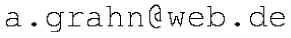
\includegraphics[height=2.7ex]{mailto}}
\maketitle

\begin{abstract}\noindent
A \LaTeX{} package for inclusion of movies, sounds and 3D objects into PDF documents with PDF-1.5/1.6 compatibility.\\[0.2\baselineskip]
\emph{Keywords}: embed, movie, LaTeX, pdfLaTeX, PDF, 3D, JavaScript, \mbox{include}, sound, video, multimedia, animation
\end{abstract}

\begin{animateinline}[autoplay,loop]{1.5}\strut{\bf\color{red} Note:}\newframe\newframe[5]\end{animateinline} This package is obsolete now. Consider using package `media9'. 
\tableofcontents

%\newpage
\section{Introduction}

The way multimedia content, i.\,e. movies and sounds, is included into PDF has changed with Adobe's PDF specification, version 1.5. PDF-1.5 supports a larger variety of movie and sound formats, limited only by the number of plug-ins available for Adobe Reader\textsuperscript{\scriptsize\textregistered}. With PDF-1.6, support for 3D objects, stored in the U3D file format, has been added. See Table \ref{table:mime} for a list of viable media formats. The specification allows media file contents to be completely embedded into the PDF output, thus producing self-contained PDF documents.

This package provides an interface to embed movies, sounds and 3D objects into PDF documents for use with \LaTeX{} as well as pdf\LaTeX. Media file contents is incorporated into PDF output by default. This is done either directly during source processing using pdf\LaTeX{} or during conversion from Postscript to PDF using Ghostscript's \verb+ps2pdf+.

The final PDF output can be viewed with Windows\textsuperscript{\scriptsize\textregistered} and Mac OS\textsuperscript{\scriptsize\textregistered} versions of Adobe Reader. However, embedded media file data can also be extracted and saved to disk from within Readers which support file attachments. This makes PDF documents a little more portable to Readers which do not ship with a multimedia plug-in.

`movie15' works well together with the presentation making package `Beamer'. In particular it supports its overlay concept. See this \href{./overlay-example.pdf}{example}.
%which uses the `Beamer' class.
Also read the comments in the example's source file, `\verb+overlay-example.tex+', on how to use `movie15' with `Beamer'.

\section{Installation}
The file `movie15.sty' should be stored in a place where \LaTeX{} can find it.

\section{Requirements}
pdf\TeX{}, version $\ge1.20$, is needed for direct PDF output.

If the package option `\verb+3D+' is set, `movie15' loads Michael Mehlich's `fp' package for fixed point arithmetic. Since it does not belong to the core packages of most \TeX{} distributions it must be installed prior to selecting the `\verb+3D+' option.

Adobe Reader, version 6, is required for playing movies and sounds, version 7 for rendering embedded 3D content.

%\newpage
\section{Using the package}
Invoke the package by putting the line
\begin{verbatim}
    \usepackage[<package options>]{movie15}
\end{verbatim}
to the preamble of your document, i.\,e. somewhere between \verb+\documentclass+ and \verb+\begin{document}+.

`movie15' honours the following package options:
\begin{verbatim}
3D
\end{verbatim}
Enables the 3D feature from the PDF-1.6 specification. Inclusion of 3D files into PDF is discussed separately in section~\ref{sec:3D}.

\begin{verbatim}
draft
\end{verbatim}
Media files are not included. Just the file name is printed in a box of size \verb+<width>+$\times$(\verb+<height>++\verb+<depth>+).
\begin{verbatim}
final
\end{verbatim}
The opposite of draft. Useful to override a global draft option specified
in the \verb+\documentclass+ command.

If PDF is generated via DVI and Postscript by the usual \verb+latex+ $\rightarrow$ \verb+dvips+ $\rightarrow$ \verb+ps2pdf+ sequence of commands, the `graphicx' package is required.

Note that several runs may be necessary to resolve internally created cross-references. Appropriate warnings will be issued in such cases.

\section{The user interface}
\subsection{Media inclusion}\label{usrif}
Movies, sounds and 3D objects are embedded into the document using the command
\begin{verbatim}
    \includemovie[<options>]{<width>}{<height>}{<media file>}
\end{verbatim}
Unless left empty, the \verb+<width>+ and \verb+<height>+ arguments must be given in valid \TeX{} dimensions. Horizontal and vertical dimensions of the media clip are scaled independently to fit \verb+<width>+ and \verb+<height>+ or, if the two latter are empty, to fit the size of the text box, given as argument to the `\verb+text+' option; see \hyperlink{lnk:textoption}{below}. \verb+<media file>+ specifies the file name of the media clip. If the media file is embedded as part of the final PDF output, which is the default, it may reside wherever \TeX{} or Ghostscript search for input files, depending on the PDF producing method.

Below, common options to \verb+\includemovie+ are listed. Options specific to embedding of 3D content are discussed separately in section~\ref{sec:3D}. The impatient reader may advance directly to the \hyperlink{sec:3Dtut}{3D quick-start guide}, which summarizes the basic steps for embedding 3D objects.
\begin{verbatim}
attach[=false]
\end{verbatim}
By default, the embedded data stream is re-used as embedded file attachment. This makes `movie15' a little more portable to PDF Readers which do not have a multimedia plug-in because it gives the user the opportunity to extract the media file and to save it to disk for later playback with an external player. However, support of file attachments is required. Re-use as file attachment can be suppressed with option `\verb+attach=false+'. Note that `\verb+attach=false+' is a poor method to prevent the user from obtaining a copy of the media file. There are several (free) tools for decompressing and extracting stream objects from PDF files.
\begin{verbatim}
autoclose
\end{verbatim}
Close the media player when the page is closed. Use of this option may be necessary for streamed media, such as Real Video.
\begin{verbatim}
autopause
\end{verbatim}
Pause playing when the page is closed.
\begin{verbatim}
autoplay
\end{verbatim}
Start playback of the media clip after the page has opened. This is especially useful if there are multiple movie clips on the current page to be played at the same time. Also resumes playback of previously paused media. In the case of embedded sound being started this way, \verb+<width>+ and \verb+<height>+ can safely be set to `0pt' since no further user interaction is necessary to start playing.
\begin{verbatim}
autostop
\end{verbatim}
Stops playing but keeps the media loaded when the page is closed. The media is rewound to its beginning or its `\verb+startat+' position. This option is set by default if neither of the options `\verb+autopause+', `\verb+autoclose+' or `\verb+continue+' is set.
\begin{verbatim}
autoresume
\end{verbatim}
Resume previously paused playback when the page is opened again.
\begin{verbatim}
continue
\end{verbatim}
Continue playback in background on premature page change. However, paused media remain paused. So do media that have reached the end or that still show the poster.
\begin{verbatim}
controls
toolbar
\end{verbatim}
Player specific controls or toolbars are displayed during playback of the media clip, if available. The default is `\verb+false+'; controls are not shown.
\begin{verbatim}
depth=<depth>
\end{verbatim}
Specifies how far the media display area should extend below the bottom line of the running text. Any valid \TeX{} dimension is accepted.
\begin{verbatim}
draft
\end{verbatim}
Locally switches to draft mode.
\begin{verbatim}
externalviewer
\end{verbatim}
Opens and plays the media in an external application.
\begin{verbatim}
final
\end{verbatim}
Locally disables draft mode.
\begin{verbatim}
inline[=false]
\end{verbatim}
Media file \emph{data} are embedded into PDF output by default.
This can be suppressed with option `\verb+inline=false+'.
\begin{verbatim}
label=<label spec>
\end{verbatim}
The media is labelled with \verb+<label spec>+ such that it can be referenced by the \verb+\movieref+ command elsewhere in the document. The \verb+\movieref+ command creates a hyperlink to either stop, pause, resume the media, to play it with different settings, such as frame rate or volume, or to show a different part of it. See section~\ref{hyperlinks} for details. \verb+<label spec>+ may consist of any sequence of letters, digits or punctuation characters.
\begin{verbatim}
mimetype=<mimetype>
\end{verbatim}
According to the PDF specification, the viewer application needs to know the MIME type of \verb+<media file>+. Package `movie15' tries to make a guess from the file name extension. If, however, a media file is of unknown type or has a non-standard file name extension, its MIME type must be explicitly specified using this option. See Table \ref{table:mime} for a list of known file name extensions.
\begin{verbatim}
mouse[=true|false]
\end{verbatim}
Enable mouse interaction: Clicking onto the media (giving it the focus) pauses the playback while clicking outside resumes it. Alternatively, once the media has got the focus, repeated pressing of key `P' on the keyboard switches between Play and Pause (at least with some players). In 3D context it specifies whether the 3D annotation should be interactive, i.\,e. responsive to mouse interaction. 3D annotations are interactive by default.
\begin{verbatim}
palindrome[=true|false]
\end{verbatim}
The media is played forward and backward, if supported by the media player. In combination with option `\verb+repeat+' this forward-and-reverse playback repeats as many times as specified. Each complete forward and reverse playback counts as one repeat.
\begin{verbatim}
playerid=<playerid>
\end{verbatim}
Forces a particular media player plug-in to be used instead of the default one. Currently, the following values are recognized:\\[1ex]
{\tt\phantom{xxxx}AAPL\_QuickTime\\
\phantom{xxxx}MACR\_FlashPlayer\\
\phantom{xxxx}RNWK\_RealPlayer\\
\phantom{xxxx}MSFT\_WindowsMediaPlayer\\
\phantom{xxxx}ADBE\_MCI} (Adobe builtin player)
\begin{verbatim}
poster
\end{verbatim}
The first frame of the movie or the frame at the beginning of the movie section specified by the `\verb+startat+' option is shown.
\begin{verbatim}
poster=<image>
\end{verbatim}
Inserts still image from file \verb+<image>+ to be shown when the media clip is not activated. The file type of \verb+<image>+ depends on the output driver: PS or EPS when using \LaTeX{} together with \verb+dvips+; PDF, PNG or JPEG when using pdf\LaTeX. This option is obsolescent and should not be used any longer. Instead, use option `\verb+text+' if a still image from an external file is to be inserted. See option `\verb+text+' for a possibility to scale the media display area according to the poster image dimensions.
\begin{verbatim}
rate=<rate>
\end{verbatim}
\verb+<rate>+ specifies the playback rate, where $1$ is normal playback, $0.5$ is half speed, $2$ is double speed, $-1$ is normal speed in reverse etc.
\begin{verbatim}
repeat[=<repeats>]
\end{verbatim}
Specifies how often the media clip or embedded 3D animation will be played. Without argument this option causes the player to repeat forever.
\begin{verbatim}
startat=<offset>
endat=<offset>
\end{verbatim}
Start/stop playback at the specified offsets. \verb+<offset>+ may be an absolute time or frame value, or a named marker, or a marker plus a time or frame. In the latter case, time or frame values are regarded as relative to the named marker. Support of markers, time and frame offsets is media type dependent. Media incompatible offsets are ignored. The following syntax applies to \verb+<offset>+:
\begin{verbatim}
    time:<time in seconds>
    frame:<frame number>
    marker:<quoted string>
\end{verbatim}
Some \verb+<offset>+ examples:
\begin{verbatim}
    time:20.5
    frame:100
    {marker:'Chapter 1', time:60}
\end{verbatim}
\hypertarget{lnk:textoption}{}
\begin{verbatim}
text=<text>
\end{verbatim}
\verb+<text>+ is typeset onto and centred within the media display area which has been specified by the \verb+<width>+ and \verb+<height>+ arguments as well as the `\verb+depth+' option. If either or both of the \verb+<width>+ and \verb+<height>+ arguments are left empty, any unspecified dimension of the media display is scaled to match the corresponding dimension, i.\,e. width and height, of \verb+<text>+. Likewise, the depth of the media display is adjusted to the depth of \verb+<text>+ if the optional `\verb+depth+' has not been given. Therefore, option `\verb+text+' can be used to scale the media display to the natural or scaled dimensions of a poster image file, such as (requires package `graphicx'; \emph{also note the empty {\tt<width>} and  {\tt<height>} arguments!}):
\begin{verbatim}
 \includemovie[text={\includegraphics[scale=2]{path/to/poster}}]
   {}{}{path/to/movie}
\end{verbatim}
In combination with the `\verb+poster+' option, which causes the poster image to be rendered from the movie during runtime, the PDF file size can be reduced somewhat by putting \verb+\includegraphics+ into a \verb+\phantom+ box:
\begin{verbatim}
   \includemovie[
     poster,
     text={\phantom{\includegraphics[scale=2]{path/to/poster}}}
   ]{}{}{path/to/movie}
\end{verbatim}
\begin{verbatim}
textoverposter[=false]
\end{verbatim}
Set this option to `\verb+false+' if you wish \verb+<text>+ to be obscured by the external poster image which has been inserted with the poster option. Deprecated.
\begin{verbatim}
url
\end{verbatim}
Treat \verb+<media file>+ as URL. Sets option `\verb+inline+' to `\verb+false+' automatically.
\begin{verbatim}
volume=<percentage of original volume>
\end{verbatim}
The meaning of this option should be self explaining.

\subsection{Inclusion of 3D objects}\label{sec:3D}
The PDF-1.6 specification, which was introduced with the advent of Adobe Acrobat/Reader 7, allows embedding of 3-dimensional graphic objects, such as CAD models or 3D scientific data, and lets the user interactively manipulate them. At the time of writing this documentation, the only supported file types were U3D~\cite{3diforg} and Adobe's PRC format, and only one commercial software~\cite{dexp} for exporting into the U3D format, yet from a number of CAD and 3D vector formats, including DXF and VRML, was known. Nevertheless, a try-out version of~\cite{dexp} can be downloaded without charge.

Selection of the `\verb+3D+' package option enables the 3D feature. Most of the command options listed in section~\ref{usrif} do what they are supposed to do in the case of embedded 3D as well. Other options are ignored, in particular `\verb+startat+', `\verb+endat+', `\verb+volume+' and `\verb+playerid+'. Options `\verb+inline=false+' and `\verb+url+' are supported, but imply option `{\tt{}ex\-ter\-nal\-view\-er}', because the 3D Reader plug-in handles embedded files only.

There are a few options to \verb+\includemovie+ which define how the 3D object is positioned within the view port of a virtual camera, or conversely, how the virtual camera is positioned and oriented within a coordinate system, called `The World', which bears the 3D object at a fixed position. Fig.~\ref{3dscene} should help to visualize the scenery: The virtual camera is orbiting at a distance of $ROO$ around the centre of orbit, specified by the position vector $\overrightarrow{COO}$; $\sphericalangle AAC$ is the camera's aperture angle. In addition, the direction vector $\overrightarrow{C2C}$ is needed to specify the initial camera position.
\begin{figure}[ht]
  \resizebox{\linewidth}{!}{\begin{picture}(0,0)%
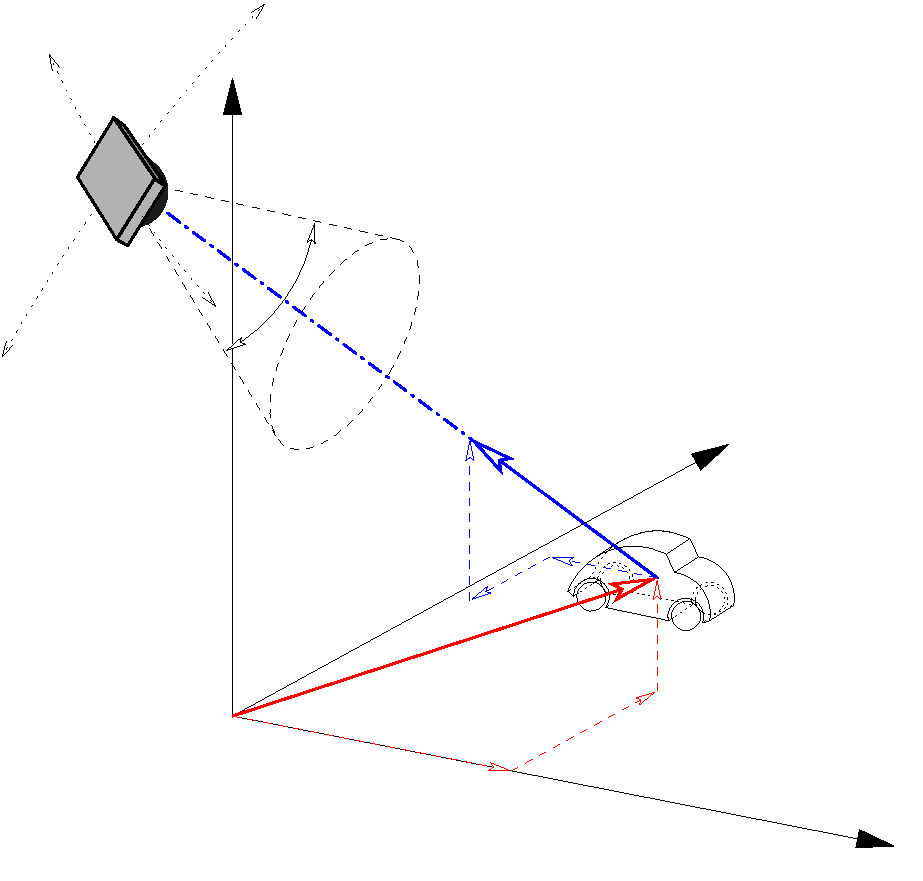
\includegraphics[clip, scale=1, viewport=0 3 433 424]{3dsystem}%
\end{picture}%
\setlength{\unitlength}{4144sp}%
%
\begingroup\makeatletter\ifx\SetFigFont\undefined%
\gdef\SetFigFont#1#2#3#4#5{%
  \reset@font\fontsize{#1}{#2pt}%
  \fontfamily{#3}\fontseries{#4}\fontshape{#5}%
  \selectfont}%
\fi\endgroup%
\begin{picture}(6873.43196911197,6682.94424710425)(435,-6534.37806949807)%
\put(4471,-3469){\makebox(0,0)[lb]{\smash{{\SetFigFont{12}{14.4}{\familydefault}{\mddefault}{\updefault}{\color[rgb]{0,0,1}$\overrightarrow{C2C}$}%
}}}}%
\put(6014,-3433){\makebox(0,0)[lb]{\smash{{\SetFigFont{12}{14.4}{\familydefault}{\mddefault}{\updefault}{\color[rgb]{0,0,0}$Y$}%
}}}}%
\put(7141,-6533){\makebox(0,0)[lb]{\smash{{\SetFigFont{12}{14.4}{\familydefault}{\mddefault}{\updefault}{\color[rgb]{0,0,0}$X$}%
}}}}%
\put(2267,-458){\makebox(0,0)[lb]{\smash{{\SetFigFont{12}{14.4}{\familydefault}{\mddefault}{\updefault}{\color[rgb]{0,0,0}$Z$}%
}}}}%
\put(4091,-4976){\makebox(0,0)[lb]{\smash{{\SetFigFont{12}{14.4}{\familydefault}{\mddefault}{\updefault}{\color[rgb]{1,0,0}$\overrightarrow{COO}$}%
}}}}%
\put(2161,-5371){\makebox(0,0)[rb]{\smash{{\SetFigFont{12}{14.4}{\familydefault}{\mddefault}{\updefault}{\color[rgb]{0,0,0}$(0,0,0)$}%
}}}}%
\put(2836,-1471){\makebox(0,0)[b]{\smash{{\SetFigFont{12}{14.4}{\familydefault}{\mddefault}{\updefault}{\color[rgb]{0,0,0}$\sphericalangle AAC$}%
}}}}%
\put(3636,-2841){\makebox(0,0)[lb]{\smash{{\SetFigFont{12}{14.4}{\familydefault}{\mddefault}{\updefault}{\color[rgb]{0,0,1}$ROO$}%
}}}}%
\end{picture}%
}
  \caption{Camera and 3D object in the World System $XYZ$; centre of orbit position vector $\vec{COO}$, centre of orbit to camera direction vector $\vec{C2C}$, radius of orbit $ROO$, aperture angle of camera $\sphericalangle AAC$.}\label{3dscene}
\end{figure}

The \emph{default view}, i.\,e. the view that is shown initially after activating the 3D object in the Reader, can be set using the options `\verb+3Dcoo+' for the centre of orbit, `\verb+3Dc2c+' for the centre of orbit to camera vector, `\verb+3Droo+' for the orbital radius and `\verb+3Daac+' for the aperture angle of the camera:
\begin{verbatim}
3Daac=<angle>
\end{verbatim}
This option sets the aperture angle of the camera, measured in degrees. Fixed point real numbers between 0 and 180 are admissible. A sensible value of 30 is pre-set by default. Larger values can be used to achieve wide-angle or fish-eye effects. See example~\ref{ex3d} in section~\ref{examples}.
\begin{verbatim}
3Dc2c=<x> <y> <z>
\end{verbatim}
\verb+<x> <y> <z>+ specify a direction vector $\overrightarrow{C2C}$ of arbitrary length, originating in the centre of orbit and pointing to the virtual camera. Only fixed point numbers in the range from\\[1ex]
\phantom{xxxx}$-999999999999999999.999999999999999999$\\
to\\
\phantom{xxxx}$+999999999999999999.999999999999999999$\\[1ex]
are allowed.
\begin{verbatim}
3Dcoo=<x> <y> <z>
\end{verbatim}
\verb+<x> <y> <z>+ specify the positional vector $\overrightarrow{COO}$ of the centre of orbit. See option `\verb+3Dc2c+' for the number format of \verb+<x> <y> <z>+.
\begin{verbatim}
3Droll=<roll>
\end{verbatim}
Prescribes an initial camera roll around the optical axis (in clockwise direction, if \verb+<roll>+ is greater that zero); measured in degrees.
\begin{verbatim}
3Droo=<r>
\end{verbatim}
\verb+<r>+ (always positive!) specifies the radius of orbit $ROO$ of the virtual camera. See option `\verb+3Dc2c+' for the number format of \verb+<r>+.

Without the above options the virtual camera sits at the origin $(0,0,0)$ of the World, looking in the positive $Y$ direction, i.\,e. default settings of \verb+3Droo=0+, \verb+3Dcoo=0 0 0+ and  \verb+3Dc2c=0 -1 0+ are assumed. (Note that $\overrightarrow{C2C}$ is the opposite of the view vector!) Thus, in order to get a `front view' of the 3D object it is sufficient to set the radius of orbit, i.\,e. the distance between camera and object appropriately. Sometimes you may want to adjust the orbital centre, i.\,e. the target of the camera as well, in particular, if the object is irregularly shaped. Fortunately, it is possible to let the values of the corresponding options be determined automatically. Simply insert a hyperlink using the \verb+\movieref+ command together with the `\verb+3Dcalculate+' option. Once the settings for `\verb+3Droo+' and `\verb+3Dcoo+' have been calculated, the hyperlink can be removed again. See section \ref{hyperlinks} for an explanation and example \ref{ex3d} in section \ref{examples}.

\begin{verbatim}
3Dbg=<r> <g> <b>
\end{verbatim}
This option sets the background colour of the canvas. Only fixed point real numbers in the range from 0 to 1 are allowed for the colour components.
\begin{verbatim}
3Dlights=<lighting scheme>
\end{verbatim}
Sets the default lighting scheme. The following values are honoured: `\verb+None+', `\verb+White+', `\verb+Day+', `\verb+Night+', `\verb+Hard+', `\verb+Primary+', `\verb+Blue+', `\verb+Red+', `\verb+Cube+', `\verb+CAD+', `\verb+HeadLamp+'. The default is to use the lighting scheme as specified within the 3D artwork.
\begin{verbatim}
3Drender=<render mode>
\end{verbatim}
\begin{flushleft}
Sets the default render mode. The following values are honoured: `\verb+Solid+', `\verb+SolidWireframe+', `\verb+Transparent+', `\verb+TransparentWireframe+', `\verb+BoundingBox+', `\verb+TransparentBoundingBox+', `\verb+TransparentBoundingBoxOutline+', `\verb+Wireframe+', `\verb+ShadedWireframe+', `\verb+HiddenWireframe+', `\verb+Vertices+', `\verb+ShadedVertices+', `\verb+SolidOutline+', `\verb+Illustration+', `\verb+ShadedIllustration+'.
\end{flushleft}

\begin{verbatim}
3Dviews=<views file>
\end{verbatim}
\emph{Deprecated}. Superseeded by the `\verb+3Dviews2+' option and a new, more flexible views file syntax (see below). File \verb+<views file>+ specifies predefined camera positions. It contains lines with the following syntax:
\begin{verbatim}
[<name>]{<coo_x> <coo_y> <coo_z>}{<c2c_x> <c2c_y> <c2c_z>}{<roo>}{<roll>}{<aac>}
\end{verbatim}
The \verb+<name>+ entry is optional. If \verb+<name>+ is not given, a default name consisting of `View' followed by the number of the current entry in the list is formed. For \verb+<coo_x>+, \verb+<coo_y>+, \verb+<coo_z>+, \verb+<c2c_x>+, \verb+<c2c_y>+, \verb+<c2c_z>+, \verb+<roo>+, \verb+<roll>+ and \verb+<aac>+ the same rules as for the corresponding options `\verb+3Dcoo+', `\verb+3Dc2c+', `\verb+3Droo+', `\verb+3Droll+' and `\verb+3Daac+' apply. Empty braces, \verb+{}+, are possible and cause default values to be used. Trailing spaces or comment signs (\%) are allowed. Reading of the file stops either at its end, at the first empty line encountered or at the first line containing nothing but spaces and/or a comment sign followed by arbitrary stuff.% See option `\verb+3Dgetview+' of \verb+\movieref+ on how to get the camera settings of the current view in the Reader, which can be used to populate a file of additional views.

\begin{verbatim}
3Dviews2=<views file>
\end{verbatim}
Instead of or in addition to the default view, further \emph{named views} can be set in an auxiliary file `\verb+<views file>+'. Besides the virtual camera position, it is possible to adjust the rendering attributes, such as visibility and transparency, of every single part in the scene. Moreover, background colour and scene lighting can be set individually for every view. The additional views can later be selected either from a drop down list in the tool bar that is associated with the activated 3D object in the Reader or from the context menu of the 3D object.

The file \verb+<views file>+ is structured into view sections, one for every view:
\begin{verbatim}
  VIEW[=<optional name>]
    COO=<coo_x> <coo_y> <coo_z>
    C2C=<c2c_x> <c2c_y> <c2c_z>
    ROO=<roo>
    AAC=<aac>
    ROLL=<roll>
    BGCOLOR=<r> <g> <b>
    RENDERMODE=<render mode>
    LIGHTS=<lighting scheme>
    PART=<part name (required) as in the Model Tree>
      VISIBLE=true | false
      OPACITY=<part opacity>
      RENDERMODE=<see option `3Drender' for possible values>
    END
    PART=<...>
      ...
    END
    etc.
  END
  VIEW
    ...
  END
  etc.
\end{verbatim}
A view section starts with the keyword \verb+VIEW+, optionally followed by a name for the view, and ends with the keyword \verb+END+. If no name is given to the view, a default one is created, consisting of `View' followed by the number of the current \verb+VIEW+ section in the file. A \verb+VIEW+ section contains optional entries for setting the camera position and global rendering attributes of the scene as well as \verb+PART+ subsections for setting rendering attributes of parts individually. Table~\ref{tab:views} lists the entries in a \verb+VIEW+ section. Part sub-sections are opened by \verb+PART=<part name>+ and closed by \verb+END+. There may be as many part subsections as there are parts a 3D object is composed of. Table~\ref{tab:parts} lists the possible entries in a \verb+PART+ sub-section. All entries are optional. \verb+<part name>+ is required and must match the part name as indicated in the Model Tree of the 3D object (accessible via right-click onto the model in the Reader). In order to avoid trouble it is recommended that part names be exclusively composed of ASCII characters. You may need to load the U3D/PRC model into the authoring application and edit the part names accordingly.

The views file can be commented. As usual with \LaTeX, comments start with the percent sign.

To facilitate the creation of a views file, a \verb+\movieref+ link with option `\verb+3Dgetview+' can be temporarily inserted into the document. When clicked, it outputs a complete \verb+VIEW+ section corresponding to the current view of the 3D object in the Reader GUI, including camera position as well as all part and viewing options that may be set via the context (right-click) menu of the 3D object. See section \ref{hyperlinks} for details.

\begin{table}
  \centering
  \caption{Entries in a {\tt VIEW} section}\label{tab:views}
  \begin{tabular}[t]{llp{0.3\linewidth}}\hline
  key & type & value\\\hline\hline
  COO & three numbers & centre of orbit, see option `{\tt 3Dcoo}'\\ 
  C2C & three numbers & centre of orbit to camera vector, see option `{\tt 3Dc2c}'\\ 
  ROO & number & radius of orbit, see option `{\tt 3Droo}'\\ 
  AAC & number & camera aperture angle, see option `{\tt 3Daac}'\\ 
  ROLL & number & camera roll, see option `{\tt 3Droll}'\\ 
  BGCOLOR & three numbers & canvas background colour (RGB), see option `{\tt 3Dbg}'\\ 
  RENDERMODE & string & render mode of the 3D object, see option `{\tt 3Drender}'\\ 
  LIGHTS & string & lighting scheme, see option `{\tt 3Dlights}'\\
  PART & sub-section & part name as in the model tree, see Table~\ref{tab:parts} for list of possible entries\\
  \hline
  \end{tabular}
\end{table}

\begin{table}
  \centering
  \caption{Entries in a {\tt PART} sub-section}\label{tab:parts}
  \begin{tabular}[t]{llp{0.3\linewidth}}\hline
  key & type & value\\\hline\hline
  VISIBLE & boolean & a flag (`{\tt true}' or `{\tt false}') indicating the visibility of this part\\
  OPACITY & number & a number between 0.0 and 1.0 specifying the opacity of this part\\
  RENDERMODE & string & rendermode of this part, overrides global {\tt RENDERMODE} value in parent {\tt VIEW} section, see option `{\tt 3Drender}'\\
  \hline
  \end{tabular}
\end{table}

\begin{verbatim}
3Djscript=<JavaScript file>
\end{verbatim}
Things like animation, lighting, background etc. may also be script driven. Option `\verb+3Djscript+' associates \verb+<JavaScript file>+ with the 3D object. The script will be executed upon activation of the object. Refer to the Acrobat 3D JavaScript Reference~\cite{jscript3D} for details. Directory `\verb+doc/javascript+' contains JavaScript example files for animation and rotation control. The files work off-the-shelf with any 3D file and may be concatenated to combine their effects.
\begin{verbatim}
3Dresource=<resource file 1>[, 3Dresource=<resource file 2> [, ...]]
\end{verbatim}
Embeds additional 3D or \emph{rasterized} image files that can be used as resources while rendering the 3D artwork. Possible file types are U3D, Postscript (\LaTeX{} + \verb+dvips+) and PDF/JPEG/PNG (pdf\LaTeX). Embedded resources must be loaded by the JavaScript method
\begin{verbatim}
  Resource('pdf://<resource path>')
\end{verbatim}
where {\tt<resource path>} stands for the path to the resource file as specified by the `\verb+3Dresource+' option. (This is just a naming convention; the files are physically embedded in the final PDF.) The following JavaScript loads an image file that was attached by `\verb+3Dresource=images/sunset.jpg+' as the background.
\begin{verbatim}
  sunset = new Image(new Resource('pdf://images/sunset.jpg')); 
  reh = new RenderEventHandler(); 
  reh.onEvent = function(event) { 
    runtime.removeEventHandler(this); 
    event.canvas.background.setImage(sunset); 
  }
  runtime.addEventHandler(reh); 
\end{verbatim}

\subsection{Media hyperlinks}\label{hyperlinks}
A movie, sound or 3D object may serve as the destination of hyperlinks, which are inserted into the document using the command
\begin{verbatim}
  \movieref[<options>]{<label spec>}{<text>}
\end{verbatim}
It makes \verb+<text>+ a hyperlink to the media that has been labelled with \verb+<label+ \verb+spec>+ using the `\verb+label+' option of the \verb+\includemovie+ command. Media hyperlinks can be inserted at any location within the document. Clicking onto the hyperlink causes the Reader to open the page containing the media it is pointing to. The primary purpose of media hyperlinks, however, is to provide a means to control the playback.

\emph{In 2D context}, clicking onto the hyperlink causes the media to stop, pause or resume, or to restart at different settings, such as frame rate, volume, starting and ending positions, depending on the \verb+<options>+ being in effect.

Options that control the playback \emph{characteristics} are: `\verb+controls+', `\verb+endat+', `\verb+mouse+', `\verb+palindrome+', `\verb+rate+', `\verb+repeat+', `\verb+startat+' and `\verb+volume+'. Their meaning is the same as for the \verb+\includemovie+ command and can be looked up in section~\ref{usrif}. Another option, `\verb+default+' causes the media to play at the original settings which were in effect during media inclusion. These options can be used in combination with the `\verb+play+' option only.

The options which follow let the hyperlink change the playback \emph{state} of media. If none of them is specified, `\verb+play+' is assumed.
\begin{verbatim}
play
\end{verbatim}
Immediately restarts playback. If new playback settings have been specified through the options given above, they override the original settings being in effect during media inclusion.
\begin{verbatim}
stop
\end{verbatim}
Stops and rewinds the media to its beginning or to the `\verb+startat+' position.
\begin{verbatim}
resume
\end{verbatim}
Resumes paused media. In fact, this option makes the hyperlink a toggle switch: repeated clicking switches between paused and resumed state.
\begin{verbatim}
pause
\end{verbatim}
Has the same effect as option `\verb+resume+'. Added for completeness only.
\begin{verbatim}
close
\end{verbatim}
Immediately closes the media player.

\emph{In 3D context}, \verb+\movieref+ can be used to define an additional view of the object, to access a particular view from the list of predefined views or to run a JavaScript. Moreover, a link can be created for calculating optimal camera settings `\verb+3Droo+' and `\verb+3Dcoo+', instead of finding them manually. The following options are recognized:
\begin{verbatim}
3Dviewindex=<index>
\end{verbatim}
Go to a predefined view of the 3D object. \verb+<index>+ can take `\verb+F+', `\verb+L+', `\verb+N+' or `\verb+P+' to access the first, last, next or previous element of the list of additional views, see option `\verb+3Dviews+' of {\tt \string\include\-movie}, or an integer specifying an index into the list. In the case of `\verb+N+' and `\verb+P+', repeated clicking onto the hyperlink allows to cycle through the list in forward or backward direction. `\verb+D+' gives access to the default view.
\begin{verbatim}
3Daac=<angle>
3Dc2c=<x> <y> <z>
3Dcoo=<x> <y> <z>
3Droll=<roll>
3Droo=<r>
\end{verbatim}
Instead of referencing an existing view of the 3D object, a new one can be defined using any of these options. See section~\ref{sec:3D}.
\begin{verbatim}
3Dcalculate[=<aac angle>]
\end{verbatim}
Mainly used during document authoring. Creates a link for calculating optimal `\verb+3Droo+' and `\verb+3Dcoo+' settings of the virtual camera, which may be used to define a default view. Clicking the link opens a dialogue box from which the settings can be copied to the clipboard for later insertion into the option list of \verb+\includemovie+. The parameter \verb+<aac angle>+ which is the camera aperture angle $\sphericalangle AAC$ used for calculation is optional. If omitted, the one set by \verb+\includemovie+ option `\verb+3Daac+' is taken.
\begin{verbatim}
3Dgetview
\end{verbatim}
Mainly used during document authoring. Camera settings as well as part and scene rendering attributes that correspond to the current view are printed to a dialogue box. The output is a readily formatted \verb+VIEWS+ section to be inserted into or appended to a file of predefined views. See option `\verb+3Dviews2+'.
\begin{verbatim}
3Djscript=<JavaScript file>
\end{verbatim}
Runs the script \verb+<JavaScript file>+ after clicking the link. Unlike the script that has been associated with the 3D annotation during object embedding, this JavaScript is not directly run by the JavaScript engine of the 3D plug-in, but is run by the Reader's own scripting engine. However, full access to the API of the 3D script engine is provided through the `\verb+context3D+' property of the `\verb+Annot3D+' object. For convenience, an associative array `\verb+annot3D+' has been provided for use within \verb+<JavaScript file>+, in order to easily access the `\verb+Annot3D+' object of the annotation the enclosing link is pointing to. The particular element of the array is referenced by the annotation's label \verb+<label spec>+, enclosed in quotation marks. As an example, the `\verb+scene+' object can be referenced within \verb+<JavaScript file>+ by
\begin{verbatim}
  annot3D['<label spec>'].context3D.scene
\end{verbatim}
For details about Acrobat JavaScript and its Annot3D object, see \cite{jscript}.

%\newpage
\subsection{Compatibility commands}
Two user commands have been provided that make `movie15' a replacement for the `multimedia' package which is part of Till Tantau's `Beamer' Class:
\begin{verbatim}
  \movie[<options>]{<poster text>}{<media file>}
\end{verbatim}
\begin{verbatim}
  \hyperlinkmovie[<options>]{<label spec>}{<text>}
\end{verbatim}
All of the optional arguments to \verb+\includemovie+ and \verb+\movieref+ can be used with the compatibility macros as well. In addition, they honour the following options:
\begin{verbatim}
height=<height of display>
width=<width of display>
\end{verbatim}
Set the horizontal and vertical dimensions of the media display area (\verb+\movie+ only).
\begin{verbatim}
autostart
\end{verbatim}
The same as `\verb+autoplay+'.
\begin{verbatim}
loop[=<repeats>]
\end{verbatim}
The same as `\verb+repeat+'.
\begin{verbatim}
once
\end{verbatim}
The same as `\verb+repeat=1+'.
\begin{verbatim}
showcontrols
\end{verbatim}
The same as `\verb+controls+'.
\begin{verbatim}
start=<offset in seconds>s
\end{verbatim}
Start playback at the specified temporal offset. The trailing `\verb+s+' is mandatory.
\begin{verbatim}
duration=<duration in seconds>s
\end{verbatim}
The duration of the media segment to be played. The trailing `\verb+s+' is mandatory. Note that `\verb+duration+' cannot be used together with option `\verb+startat+' from \verb+\includemovie+. In order to define a media segment options can be combined as follows: `\verb+startat+'/`\verb+endat+', `\verb+start+'/`\verb+endat+', `\verb+start+'/`\verb+duration+'.

%\newpage
\section{Examples}\label{examples}
\begin{enumerate}
\item A short circular MPEG movie, taken from \href{http://www.linux-video.net/Samples/}{\tt http://www.linux-video.net/} \href{http://www.linux-video.net/Samples/}{\tt Samples/}

\begin{minipage}{0.5\linewidth}
{\tt%
  \string\includemovie[\\
  \phantom{xx}poster,\\
  \phantom{xx}text=(random.mpg),\\
  \phantom{xx}mouse,\\
  \phantom{xx}repeat\\
  ]\string{\\
  \phantom{xx}.5\string\linewidth\\
  \string}\string{\\
  \phantom{xx}.375\string\linewidth\\
  \string}\string{random.mpg\string}
}
\end{minipage}%
\begin{minipage}{0.5\linewidth}
\begin{center}
  \includemovie[poster, text=(random.mpg), mouse, repeat]{\linewidth}{.75\linewidth}{random.mpg}
\end{center}
\end{minipage}

%\newpage
\item Another MPEG movie, loaded on the fly from \href{http://www.linux-video.net/Samples/}{\tt http://www.linux-video} \href{http://www.linux-video.net/Samples/}{\tt .net/Samples/}. Hence, a working Internet connection is required. This time, we force the QuickTime plug-in to be used instead of MediaPlayer (Windows boxes only). Well, the latter seems to be bugged. Quod erat expectandum.

\begin{minipage}{0.5\linewidth}
{\tt%
  \string\includemovie[\\
  \phantom{xx}poster,\\
  \phantom{xx}label=alien,\\
  \phantom{xx}text=(AlienSong.mpg),\\
  \phantom{xx}url,\\
  \phantom{xx}playerid=AAPL\_QuickTime,\\
  \phantom{xx}repeat\\
  ]\string{\\
  \phantom{xx}.5\string\linewidth\\
  \string}\string{\\
  \phantom{xx}.375\string\linewidth\\
  \string}\string{http://www.linux-video.net/Samples/Mpeg1/AlienSong.mpg\string}\\
  \string\movieref[rate=0.5]\string{alien\string}\string{Slow\string}\\
  \string\movieref[default]\string{alien\string}\string{Normal\string}\\
  \string\movieref[rate=2]\string{alien\string}\string{Fast\string}\\
  \string\movieref[pause]\string{alien\string}\string{Play/Pause\string}\\
  \string\movieref[stop]\string{alien\string}\string{Stop\string}
}
\end{minipage}%
\begin{minipage}{0.5\linewidth}
\begin{center}
  \includemovie[
    poster,
    label=alien,
    text=(AlienSong.mpg),
    repeat,
    playerid=AAPL_QuickTime,
    url
  ]{\linewidth}{.75\linewidth}{http://www.linux-video.net/Samples/Mpeg1/AlienSong.mpg}\\
% ]{\linewidth}{.75\linewidth}{AlienSong.mpg}\\
\movieref[rate=0.5]{alien}{Slow}\hfill
\movieref[default]{alien}{Normal}\hfill
\movieref[rate=2]{alien}{Fast}\hfill
\movieref[pause]{alien}{Play/Pause}\hfill
\movieref[stop]{alien}{Stop}\vspace{19 ex}
\end{center}
\end{minipage}

%\newpage
\item\label{ex3d} Embedded U3D file. It is based on a VRML model by Peter Whitehouse, \href{http://www.wonko.info/vrml/index.htm}{\tt http://www.wonko.info/vrml/index.htm}. Conversion to U3D has been made with DeepExploration\textsuperscript{\scriptsize\textregistered}\cite{dexp}. The file `{\tt dice.vws}' provides predefined views to be selected from the 3D toolbar or by right click.% The JavaScript `{\tt turntable.js}' disables the annoying Gimbal rotation mode.

\begin{minipage}[b]{0.5\linewidth}
{\tt%
  \string\includemovie[\\
  \phantom{xx}poster,\\
  \phantom{xx}toolbar,\\
  \phantom{xx}label=dice,\\
  \phantom{xx}text=(dice.u3d),\\
  \phantom{xx}3Droo=27,\\
  \phantom{xx}3Dlights=Cube,\\
  \phantom{xx}3Djscript=turntable.js,\\
  \phantom{xx}3Dviews2=dice.vws\\
  ]\string{\\
  \phantom{xx}.5\string\linewidth\\
  \string}\string{\\
  \phantom{xx}.5\string\linewidth\\
  \string}\string{dice.u3d\string}\\
  \string\movieref[\\
  \phantom{xx}3Dviewindex=N\\
  ]\string{dice\string}\string{Click here\string} \dots\\
  \string\movieref[\\
  \phantom{xx}3Dcalculate=60\\
  ]\string{dice\string}\string{This link\string} \dots
}
\end{minipage}%
\begin{minipage}[b]{0.5\linewidth}
\begin{center}
  \includemovie[
    poster,
    toolbar, %same as `controls'
    label=dice,
    text=(dice.u3d),
    3Droo=27,
    3Dlights=Cube,
    3Dviews2=dice.vws,
    3Djscript=turntable.js
  ]{\linewidth}{\linewidth}{dice.u3d}
\end{center}
\movieref[3Dviewindex=N]{dice}{Click here} to cycle through the list of predefined views. \movieref[3Dcalculate=60]{dice}{This link} calculates 3D option settings for a 60\textdegree{} aperture angle of the virtual camera.
\end{minipage}

\end{enumerate}

%\newpage
\appendix
\section{3D quick-start guide}\hypertarget{sec:3Dtut}{}
\begin{enumerate}
  \item Insert the 3D object with default camera settings and a {\tt \string\movieref} referencing it:

  {\tt%
    \string\includemovie[poster, label=my\_label]\string{\\
    \phantom{xx}.5\string\linewidth\\
    \string}\string{\\
    \phantom{xx}.5\string\linewidth\\
    \string}\string{\\
    \phantom{xx}my\_file.u3d\\
    \string}\string\\\\
    \string\movieref[3Dcalculate]\string{my\_label\string}\string{Click here!\string}
  }

  \item Compile and recompile the document until no more `movie15' related warnings appear.
  \item Open the PDF document in Adobe Reader and go to the page containing the 3D object. Click the link and wait for a dialogue box to pop up. Optionally, drag the object with the mouse to change the viewpoint of the camera (the dialogue must be closed beforehand) and click the link again.
  \item Copy the settings ({\tt 3Droo=...}, {\tt 3Dcoo=...}, etc.) from the dialogue box into the option list of {\tt \string\include\-movie}. Remove the link from the document source:

  {\tt%
    \string\includemovie[\\
    \phantom{xx}poster, 3Droo=33.3333, 3Dcoo=1.2345 9.8765 0\\
    ]\string{\\
    \phantom{xx}.5\string\linewidth\\
    \string}\string{\\
    \phantom{xx}.5\string\linewidth\\
    \string}\string{\\
    \phantom{xx}my\_file.u3d\\
    \string}
  }

  \item Again, compile and recompile the document until no more `movie15' related warnings appear.
  \xdef\lastcount{\theenumi}
\end{enumerate}

\emph{Optional steps:}

\begin{enumerate}
  \setcounter{enumi}{\lastcount}
  \item Create a file with predefined views of the 3D object and attach it to the latter using the `{\tt{}3Dviews2}' option:

  {\tt%
    \string\includemovie[\\
    \phantom{xx}..., label=my\_label, 3Dviews2=my\_views.vws\\
    ]\string{\\
    \phantom{xx}.5\string\linewidth\\
    \string}\string{\\
    \phantom{xx}.5\string\linewidth\\
    \string}\string{\\
    \phantom{xx}my\_file.u3d\\
    \string}
  }

  The views file can easily be populated using a temporarily inserted {\tt \string\movie\-ref} link:

  {\tt%
    \string\movieref[3Dgetview]\string{my\_label\string}\string{Click here!\string}
  }

  Manipulate the 3D object using the mouse and any of the `Part' and `Viewing' options from the 3D context menu in the Reader. Visibility, lighting, transparency, render mode etc. of individual parts or of the object as a whole can be changed this way. Sometimes you may wish to move the camera target into the centre of a single part or of a group of visible parts. The context menu items `Part Options$\rightarrow$Zoom to Part' and `Part Options$\rightarrow$Fit Visible' can be used for this purpose.
  
  When you are done, click the link to get the {\tt VIEW} section, readily formatted for insertion into the views file. Repeat this procedure to get any number of views you want to predefine. The views file can be edited manually to give meaningful names to the views (change the value of the {\tt VIEW} entry) or to further tweak camera settings, opacity etc.

  If you are satisfied with the predefined views in the views file, the default view first specified through the options of {\tt\string\includemovie} can be deleted. The first view in the views file becomes the default view then.

  \item Associate a JavaScript with the 3D object:

  {\tt%
    \string\includemovie[\\
    \phantom{xx}..., 3Djscript=my\_script.js\\
    ]\string{\\
    \phantom{xx}.5\string\linewidth\\
    \string}\string{\\
    \phantom{xx}.5\string\linewidth\\
    \string}\string{\\
    \phantom{xx}my\_file.u3d\\
    \string}
  }

  JavaScript is \emph{not} required to make use of \emph{embedded} keyframe animation. Just click the `Play' button in the 3D toolbar of the 3D annotation. However, the example file `{\tt{}animation.js}' in the `{\tt{}doc/javascript}' directory provides additional controls (accessible via the context menu of the 3D annotation) that can be used to change the speed of a running animation. The `Up', `Down' and `Home' keys of the keyboard can also be used.
  
  Another useful example file you may want to experiment with is `{\tt{}turn\-table.js}'. It improves the rotational behaviour of the 3D object, because it prevents the object from tilting to the side while dragging the mouse.

  All files in `{\tt{}doc/javascript}' work off-the-shelf and can be copied into a single file in order to combine their effects.

\end{enumerate}

\section{Media formats}
\begin{table}[H]
\caption{Media formats for use with Adobe Reader (partially from \cite{pdfspec})}\label{table:mime}
\RaggedRight
\begin{tabular}[t]{llp{0.36\linewidth}}\hline
Extension & MIME type & Description\\\hline\hline\\[-2.5ex]
aif, aifc, aiff & audio/aiff & Audio Interchange File Format\\
au, snd         & audio/basic & NeXT/Sun Audio Format\\
avi             & video/avi & Audio/Video Interleaved\\
gif             & image/gif & (animated) GIF\\
mid, rmi        & audio/midi & Musical Instrument Digital Interface\\
mov, qt         & video/quicktime & Apple QuickTime\\
mp3, m3u        & audio/x-mp3 & MPEG Audio Layer-3\\
mp4             & video/mp4 & MPEG-4 Video\\
mpeg, mpg       & video/mpeg & MPEG-1 \& 2 Video\\
prc             & model/prc  & Adobe PRC Format (3D), requires Reader-8.1 or higher\\
ra              & audio/vnd.rn-realaudio & Real Audio\\
rm, rv          & application/vnd.rn-realmedia & Real Media (video \& sound)\\
smil            & application/smil & Synchronized Multimedia Integration Language\\
swf             & application/x-shockwave-flash & (Adobe?) Macromedia Flash\\
u3d             & model/u3d  & Universal 3D File Format\\
wav             & audio/wav  & MS Audio Format\\
wma             & audio/x-ms-wma & Windows Media Audio\\
wmv             & video/x-ms-wmv & Windows Media Video\\\hline
\end{tabular}
\end{table}

\begin{thebibliography}{9}
  \bibitem{pdfspec} Adobe Systems Inc.: \emph{PDF Reference, fifth edition: Adobe Portable Document Format version 1.6}, 2004, Implementation note 144, Appendix H.3, available at \href{http://www.adobe.com/devnet/pdf/pdf_reference.html}{\tt http://www.adobe.com/devnet/pdf/pdf\_reference.html}
  \bibitem{3diforg} \href{http://www.3dif.org/}{\tt http://www.3dif.org/}
  \bibitem{dexp} \href{http://www.righthemisphere.com/products/dexp/}{\tt http://www.righthemisphere.com/products/dexp/}
  \bibitem{jscript3D}  Adobe Systems Inc.: \emph{JavaScript for Acrobat\textsuperscript{\scriptsize\textregistered} 3D Annotations API Ref\-er\-ence}, 2006, available at \href{http://www.adobe.com/devnet/acrobat/javascript3d.html}{\tt http://www.adobe.com/devnet/acrobat/} \href{http://www.adobe.com/devnet/acrobat/javascript3d.html}{\tt javascript3d.html}
  \bibitem{jscript}  Adobe Systems Inc.: \emph{JavaScript for Acrobat\textsuperscript{\scriptsize\textregistered} API Reference}, 2006, available at \href{http://www.adobe.com/devnet/acrobat/javascript.html}{\tt http://www.adobe.com/devnet/acrobat/javascript.html}
\end{thebibliography}

\end{document}
